\documentclass{beamer}

% Packages
\usepackage[utf8]{inputenc}
\usepackage[T1]{fontenc}
\usepackage{lmodern}
\usepackage{amsmath, amssymb}
\usepackage{graphicx}
\usepackage{hyperref}
\usepackage{tikz}
\usepackage{pgfplots}
\usepackage{xcolor}
\usepackage{listings}

\definecolor{codegreen}{rgb}{0,0.6,0}
\definecolor{codegray}{rgb}{0.5,0.5,0.5}
\definecolor{codepurple}{rgb}{0.58,0,0.82}
\definecolor{backcolour}{rgb}{0.95,0.95,0.92}

\lstdefinestyle{mystyle}{
    backgroundcolor=\color{backcolour},   
    commentstyle=\color{codegreen},
    keywordstyle=\color{magenta},
    numberstyle=\tiny\color{codegray},
    stringstyle=\color{codepurple},
    basicstyle=\ttfamily\footnotesize,
    breakatwhitespace=false,         
    breaklines=true,                 
    captionpos=b,                    
    keepspaces=true,                 
    numbers=left,                    
    numbersep=5pt,                  
    showspaces=false,                
    showstringspaces=false,
    showtabs=false,                  
    tabsize=2
}

\lstset{style=mystyle}

\pgfplotsset{compat=1.18}

% set style to berlin
\usetheme{Berlin}
% Title and author information
\title{Python Package Managers for Research Project}
\author{Zesen Zhuang}
\institute{SciEcon CIC}
\date{\today}

% Document
\begin{document}

% Title slide
\begin{frame}
  \titlepage
\end{frame}

% Table of contents
\begin{frame}
  \frametitle{Outline}
  \tableofcontents
\end{frame}

\section{What it is and why}

\begin{frame}
  \frametitle{What is Package Manager and Why}

  A Python environment manager is a tool that allows you to create and manage separate Python environments on your system. This can be useful for several reasons:

  \begin{itemize}
    \item It allows you to have multiple versions of Python installed on your system and switch between them easily.
    \item It allows you to install and manage packages in a specific environment, rather than globally on your system. This can be useful for isolating different projects or environments, and for avoiding conflicts between package versions.
    \item It allows you to create and share reproducible environments, which can be useful for collaborating with others or for deploying Python applications.
  \end{itemize}

\end{frame}

\section{Frequently used managers}

\begin{frame}
  \frametitle{Some Examples}

  Frequently used \texttt{Python} package manager

  \begin{itemize}
    \item \texttt{pip}: \url{https://pypi.org/project/pip/}
    \item \texttt{conda}: \url{https://docs.conda.io/en/latest/}
    \item \texttt{virtualenv}: \url{https://virtualenv.pypa.io/en/latest/}
    \item \texttt{pyenv}: \url{https://github.com/pyenv/pyenv}
    \item \texttt{pipenv}: \url{https://pipenv.pypa.io/en/latest/}
  \end{itemize}

\end{frame}

\section{Details}

\subsection{\texttt{pip}}

% References
\begin{frame}[fragile]
  \frametitle{\texttt{pip}}
  \texttt{pip} is the default package manager for Python, and it is included with most Python installations.

  Here are some common tasks you can perform using \texttt{pip}:

  \begin{lstlisting}
pip install numpy # install a package 
pip install --upgrade numpy # upgrade a package
pip uninstall numpy # uninstall a package
pip list # list installed packages
pip freeze > requirements.txt # save installed packages to a file
pip install -r requirements.txt # install packages from a file
\end{lstlisting}

\end{frame}

\subsection{conda}

\begin{frame}
  \frametitle{\texttt{conda}}

  \texttt{conda} is a package manager and environment manager developed by Anaconda, Inc. It is particularly useful for scientific computing and data science, and it can be used to create, manage, and share Python environments and packages.

  Here are some common tasks you can perform using \texttt{conda}.
  \begin{itemize}
    \item Create a new environment
    \item Activate an environment
    \item Deactivate an environment
    \item Install a package
    \item Upgrade a package
    \item Uninstall a package
    \item List environments
    \item Export an environment
  \end{itemize}

\end{frame}

\begin{frame}[fragile]
  \frametitle{\texttt{conda} continued}

  Create a new environment: To create a new environment using conda, you can use the conda create command followed by the name of the environment and the packages you want to include in it. For example, to create an environment named myenv with Python 3.8 and the numpy package, you can use the following command:

  \begin{lstlisting}
conda create --name myenv python=3.8 numpy
\end{lstlisting}

\end{frame}

\begin{frame}[fragile]
  \frametitle{\texttt{conda} continued}

  Activate an environment: To activate an environment, you can use the conda activate command followed by the name of the environment. For example:

  \begin{lstlisting}
conda activate myenv
\end{lstlisting}

  \begin{figure}[ht]
    \centering
    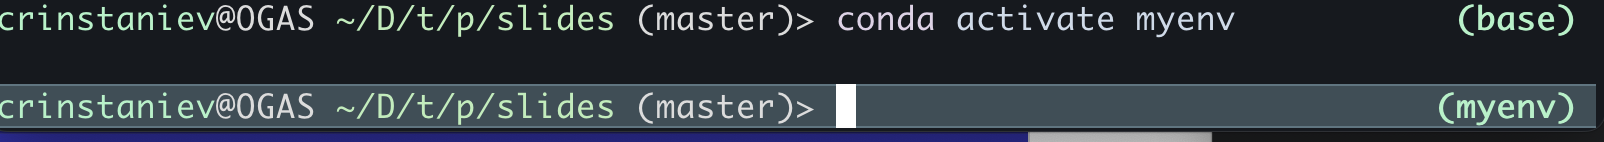
\includegraphics[width=0.8\textwidth]{imgs/conda_activated.png}
    \caption{\texttt{conda} activated}
  \end{figure}

  As shown in figure above, the environment name is displayed in parentheses in the prompt.

\end{frame}

\begin{frame}[fragile]
  \frametitle{\texttt{conda} continued}

  Deactivate an environment: To deactivate the current environment, you can use the conda deactivate command.

  \begin{lstlisting}
conda deactivate
\end{lstlisting}

\end{frame}

\begin{frame}[fragile]
  \frametitle{\texttt{conda} continued}

  Install a package: To install a package in the current environment, you can use the conda install command followed by the name of the package. For example:

  \begin{lstlisting}
conda install numpy
\end{lstlisting}

  Upgrade a package: To upgrade an installed package to the latest version, you can use the conda update command followed by the name of the package. For example:

  \begin{lstlisting}
conda update numpy
\end{lstlisting}

  Uninstall a package: To uninstall a package, you can use the conda remove command followed by the name of the package. For example:

  \begin{lstlisting}
conda remove numpy
\end{lstlisting}

\end{frame}



\begin{frame}[fragile]
  \frametitle{\texttt{conda} continued}

  List environments: To see a list of all the environments on your system, you can use the conda env list command.

  \begin{lstlisting}
conda env list
\end{lstlisting}

  Export an environment: To create a YAML file that describes the current environment and its packages, you can use the conda env export command. This can be useful for creating a reproducible environment or for sharing your environment with others.

  \begin{lstlisting}
conda env export > environment.yml
\end{lstlisting}

\end{frame}

\subsection{virtualenv}

\begin{frame}[fragile]
  \frametitle{\texttt{virtualenv}}

  virtualenv is a tool that allows you to create isolated Python environments. It can be useful for testing and deploying Python applications, as it allows you to create environments with specific package versions and configurations.

\end{frame}

\begin{frame}[fragile]
  \frametitle{\texttt{virtualenv} continued}

  Install virtualenv: To use virtualenv, you will first need to install it using pip. You can do this by running the following command:

  \begin{lstlisting}
pip install virtualenv
\end{lstlisting}

  Create a new environment: To create a new environment using virtualenv, you can use the virtualenv command followed by the name of the environment. For example, to create an environment named myenv, you can use the following command:

  \begin{lstlisting}
virtualenv myenv
\end{lstlisting}

\end{frame}

\begin{frame}[fragile]
  \frametitle{\texttt{virtualenv} continued}

  Activate an environment: To activate an environment, you will need to use the activate script located in the bin directory of the environment. On Windows, you can do this by running the following command:

  \begin{lstlisting}
myenv\Scripts\activate.bat
\end{lstlisting}

  On macOS or Linux, you can do this by running the following command:

  \begin{lstlisting}
source myenv/bin/activate
\end{lstlisting}

  Deactivate an environment: To deactivate the current environment, you can use the deactivate command.

  \begin{lstlisting}
deactivate
\end{lstlisting}

\end{frame}

\begin{frame}[fragile]
  \frametitle{\texttt{virtualenv} continued}

  Install a package: To install a package in the current environment, you can use pip as usual. For example:

  \begin{lstlisting}
pip install numpy
\end{lstlisting}

  Create a requirements file: To create a requirements file that lists all the packages and their versions installed in the current environment, you can use the pip freeze command. This can be useful for creating a reproducible environment or for sharing your dependencies with others.

  \begin{lstlisting}
pip freeze > requirements.txt
\end{lstlisting}

\end{frame}

\subsection{\texttt{pyenv}}

\begin{frame}
  \frametitle{\texttt{pyenv}}

  pyenv is a tool that allows you to manage multiple Python versions and switch between them easily. It can also be used to create and manage virtual environments.

\end{frame}

\begin{frame}[fragile]
  \frametitle{\texttt{pyenv} continued}

  Install pyenv: To use pyenv, you will first need to install it. You can do this by following the instructions on the pyenv GitHub page: \url{https://github.com/pyenv/pyenv#installation}

  List available Python versions: To see a list of all the Python versions that are available to pyenv, you can use the pyenv install --list command.

  \begin{lstlisting}
pyenv install --list
\end{lstlisting}

  Install a Python version: To install a specific Python version using pyenv, you can use the pyenv install command followed by the version number. For example, to install Python 3.9, you can use the following command:

  \begin{lstlisting}
pyenv install 3.9
\end{lstlisting}

\end{frame}

\begin{frame}[fragile]
  \frametitle{\texttt{pyenv} continued}

  Set the global Python version: To set the global Python version, which will be used as the default Python version for all your terminal sessions, you can use the pyenv global command followed by the version number. For example:

  \begin{lstlisting}
pyenv global 3.9
\end{lstlisting}

  Create a new virtual environment: To create a new virtual environment using pyenv, you can use the pyenv virtualenv command followed by the name of the environment and the Python version you want to use. For example, to create an environment named myenv using Python 3.9, you can use the following command:

  \begin{lstlisting}
pyenv virtualenv 3.9 myenv
\end{lstlisting}

\end{frame}

\begin{frame}[fragile]
  \frametitle{\texttt{pyenv} continued}

  Create a new virtual environment: To create a new virtual environment using pyenv, you can use the pyenv virtualenv command followed by the name of the environment and the Python version you want to use. For example, to create an environment named myenv using Python 3.9, you can use the following command:

  \begin{lstlisting}
pyenv virtualenv 3.9 myenv
\end{lstlisting}

  Activate a virtual environment: To activate a virtual environment, you can use the pyenv activate command followed by the name of the environment. For example:

  \begin{lstlisting}
pyenv activate myenv
\end{lstlisting}

\end{frame}

\begin{frame}[fragile]
  \frametitle{\texttt{pyenv} continued}

  Deactivate a virtual environment: To deactivate the current virtual environment, you can use the pyenv deactivate command.

  \begin{lstlisting}
pyenv deactivate
\end{lstlisting}

\end{frame}

\subsection{\texttt{pipenv}}
\begin{frame}
  \frametitle{\texttt{pipenv}}

  pipenv is a tool that combines pip and virtualenv into a single package, and it is designed to make it easier to manage Python environments and packages.

\end{frame}

\begin{frame}[fragile]
  \frametitle{\texttt{pipenv} continued}

  Install pipenv: To use pipenv, you will first need to install it using pip. You can do this by running the following command:

  \begin{lstlisting}
pip install pipenv
\end{lstlisting}

  Create a new environment: To create a new environment and install the packages specified in a Pipfile using pipenv, you can use the pipenv install command. For example:
  \begin{lstlisting}
pipenv install
\end{lstlisting}

\end{frame}

\begin{frame}[fragile]
  \frametitle{\texttt{pipenv} continued}

  Install a package: To install a package and add it to the Pipfile using pipenv, you can use the pipenv install command followed by the name of the package. For example:

  \begin{lstlisting}
pipenv install numpy
\end{lstlisting}

  Upgrade a package: To upgrade an installed package to the latest version and update the Pipfile accordingly, you can use the pipenv update command followed by the name of the package. For example:

  \begin{lstlisting}
pipenv update numpy
\end{lstlisting}

\end{frame}

\begin{frame}[fragile]
  \frametitle{\texttt{pipenv} continued}

  Uninstall a package: To uninstall a package and remove it from the Pipfile, you can use the pipenv uninstall command followed by the name of the package. For example:

  \begin{lstlisting}
pipenv uninstall numpy
\end{lstlisting}

  Activate the environment: To activate the environment created by pipenv, you can use the pipenv shell command. This will open a new shell with the environment activated.

  \begin{lstlisting}
pipenv shell
\end{lstlisting}

  Deactivate the environment: To deactivate the current environment, you can use the exit command.

  \begin{lstlisting}
exit
\end{lstlisting}

\end{frame}

\section{End}
\begin{frame}
  \LARGE
  \centering
  Thanks for listening!
\end{frame}

\end{document}

